%!TEX program = pdflatex
\documentclass[UTF8]{ctexart}

\usepackage[a4paper, scale=.8]{geometry}
\usepackage{graphicx} 
\usepackage{paralist}

\pagestyle{empty}
\ctexset{
    section/format+ = \raggedright
}

\title{第三方在线支付协议形式化验证}
\author{xxx}

\begin{document}
\maketitle
\section{关键词}
% 描述研究领域、方法、技术等的专业词汇
支付安全，安全协议，在线支付，形式化验证

\section{背景}
\subsection{应用场景}
% 使用文字或图像描绘论文的应用场景，建议150字以下
第三方支付已成为国内最主流的支付方式。
据调研，2023年，中国个人第三方移动支付交易规模达到63.6万亿元人民币，其中线上场景支付为32.2万亿元人民币，占比超50\%\cite{Iresearch2024-report}。
然而，以微信和支付宝为首的第三方支付平台的安全性高度依赖商户、用户自身的安全防护能力，
支付链路中任一环节（如商户服务器、用户网络环境）的漏洞均可能引发资金风险，形成典型的``木桶效应''。
当前，支付平台主要承担支付通道功能，而未能在支付全链路上承担起应有的主导责任。
支付平台应当充分利用其技术优势，在协议设计中充分考虑用户在非可信环境中的支付安全需求，而非完全将安全责任下放给防护能力参差不齐的商户和用户。
特别是在开放网络环境下，商户系统和用户终端往往缺乏专业的安全防护措施，这种责任划分方式显然存在重大安全隐患。
因此，亟需分析现有第三方在线支付协议的安全性，并提出一种安全的、可验证的支付协议，以提升支付过程的安全性和透明度。 


\subsection{问题陈述}
% 陈述在该场景中存在的安全、隐私、效率等问题，建议150字以下
\textbf{核心问题：}支付 APP 执行支付操作时未认证支付信息的完整性和真实性，攻击者可篡改支付信息发起欺诈交易。
现有的第三方支付协议存在三大潜在的\textbf{攻击场景：}
\begin{itemize}
    \item \textbf{商户品牌名关联性缺陷：}（收款方混淆）\newline
        由于支付界面显示的商家公司名称与消费者认知的品牌名称存在信息不对称，用户难以核实收款方身份。
        如在游戏平台``Steam''购买游戏时，实际收款账户为其公司名``Valve''，二者名称存在显著差异。
        这为攻击者创造了条件：其可通过篡改收款账户诱导用户向非法主体付款（如``Value''），而用户在此过程中无法进行有效的关联性校验。
    \item \textbf{订单金额替换漏洞}：（支付金额混淆）\newline
        在使用手机应用跳转支付场景中，商户APP转移到后台，前台显示支付软件。
        由于支付软件界面未同步显示原商城的订单明细，攻击者将支付订单替换为金额相似的订单（如将99.81元的订单改为99.87元的订单）。
        用户难以察觉细微差异，尤其在动态金额场景（如运费计算、活动优惠）。
    \item \textbf{同商品订单替换攻击}:（下单用户混淆）\newline
        在此场景中，当用户于平台下单后，攻击者会平行下单购买相同商品，并将用户的支付请求劫持并指向攻击者的订单。
        其结果是，用户在不知情的情况下为攻击者的订单完成了支付。
        由于商品名称、支付金额及收款方信息均完全一致，该攻击极具隐蔽性，用户难以识别。
\end{itemize}

\textbf{攻击验证：} 我们调研发现，Android 上基于 Intent 的支付调起存在安全隐患：
微信、支付宝均支持通过隐式 Intent 接收支付请求，恶意应用可声明相同的 Scheme 劫持请求，从而篡改支付参数并诱发欺诈交易。
图~\ref{fig:wechat_android_attack}展示微信 Android 端支付隐式 Intent 调用劫持攻击示意图，针对支付宝的攻击类似。

我们初步调查了14款APP，发现其中5款存在上述安全问题。
此外还观察到一种现象：
部分漏洞仅出现在新版本中，而旧版本中并不存在。这表明开发者可能并未充分意识到支付软件的隐式 intent 调用存在安全隐患。

\begin{figure}[!h]
    \centering
    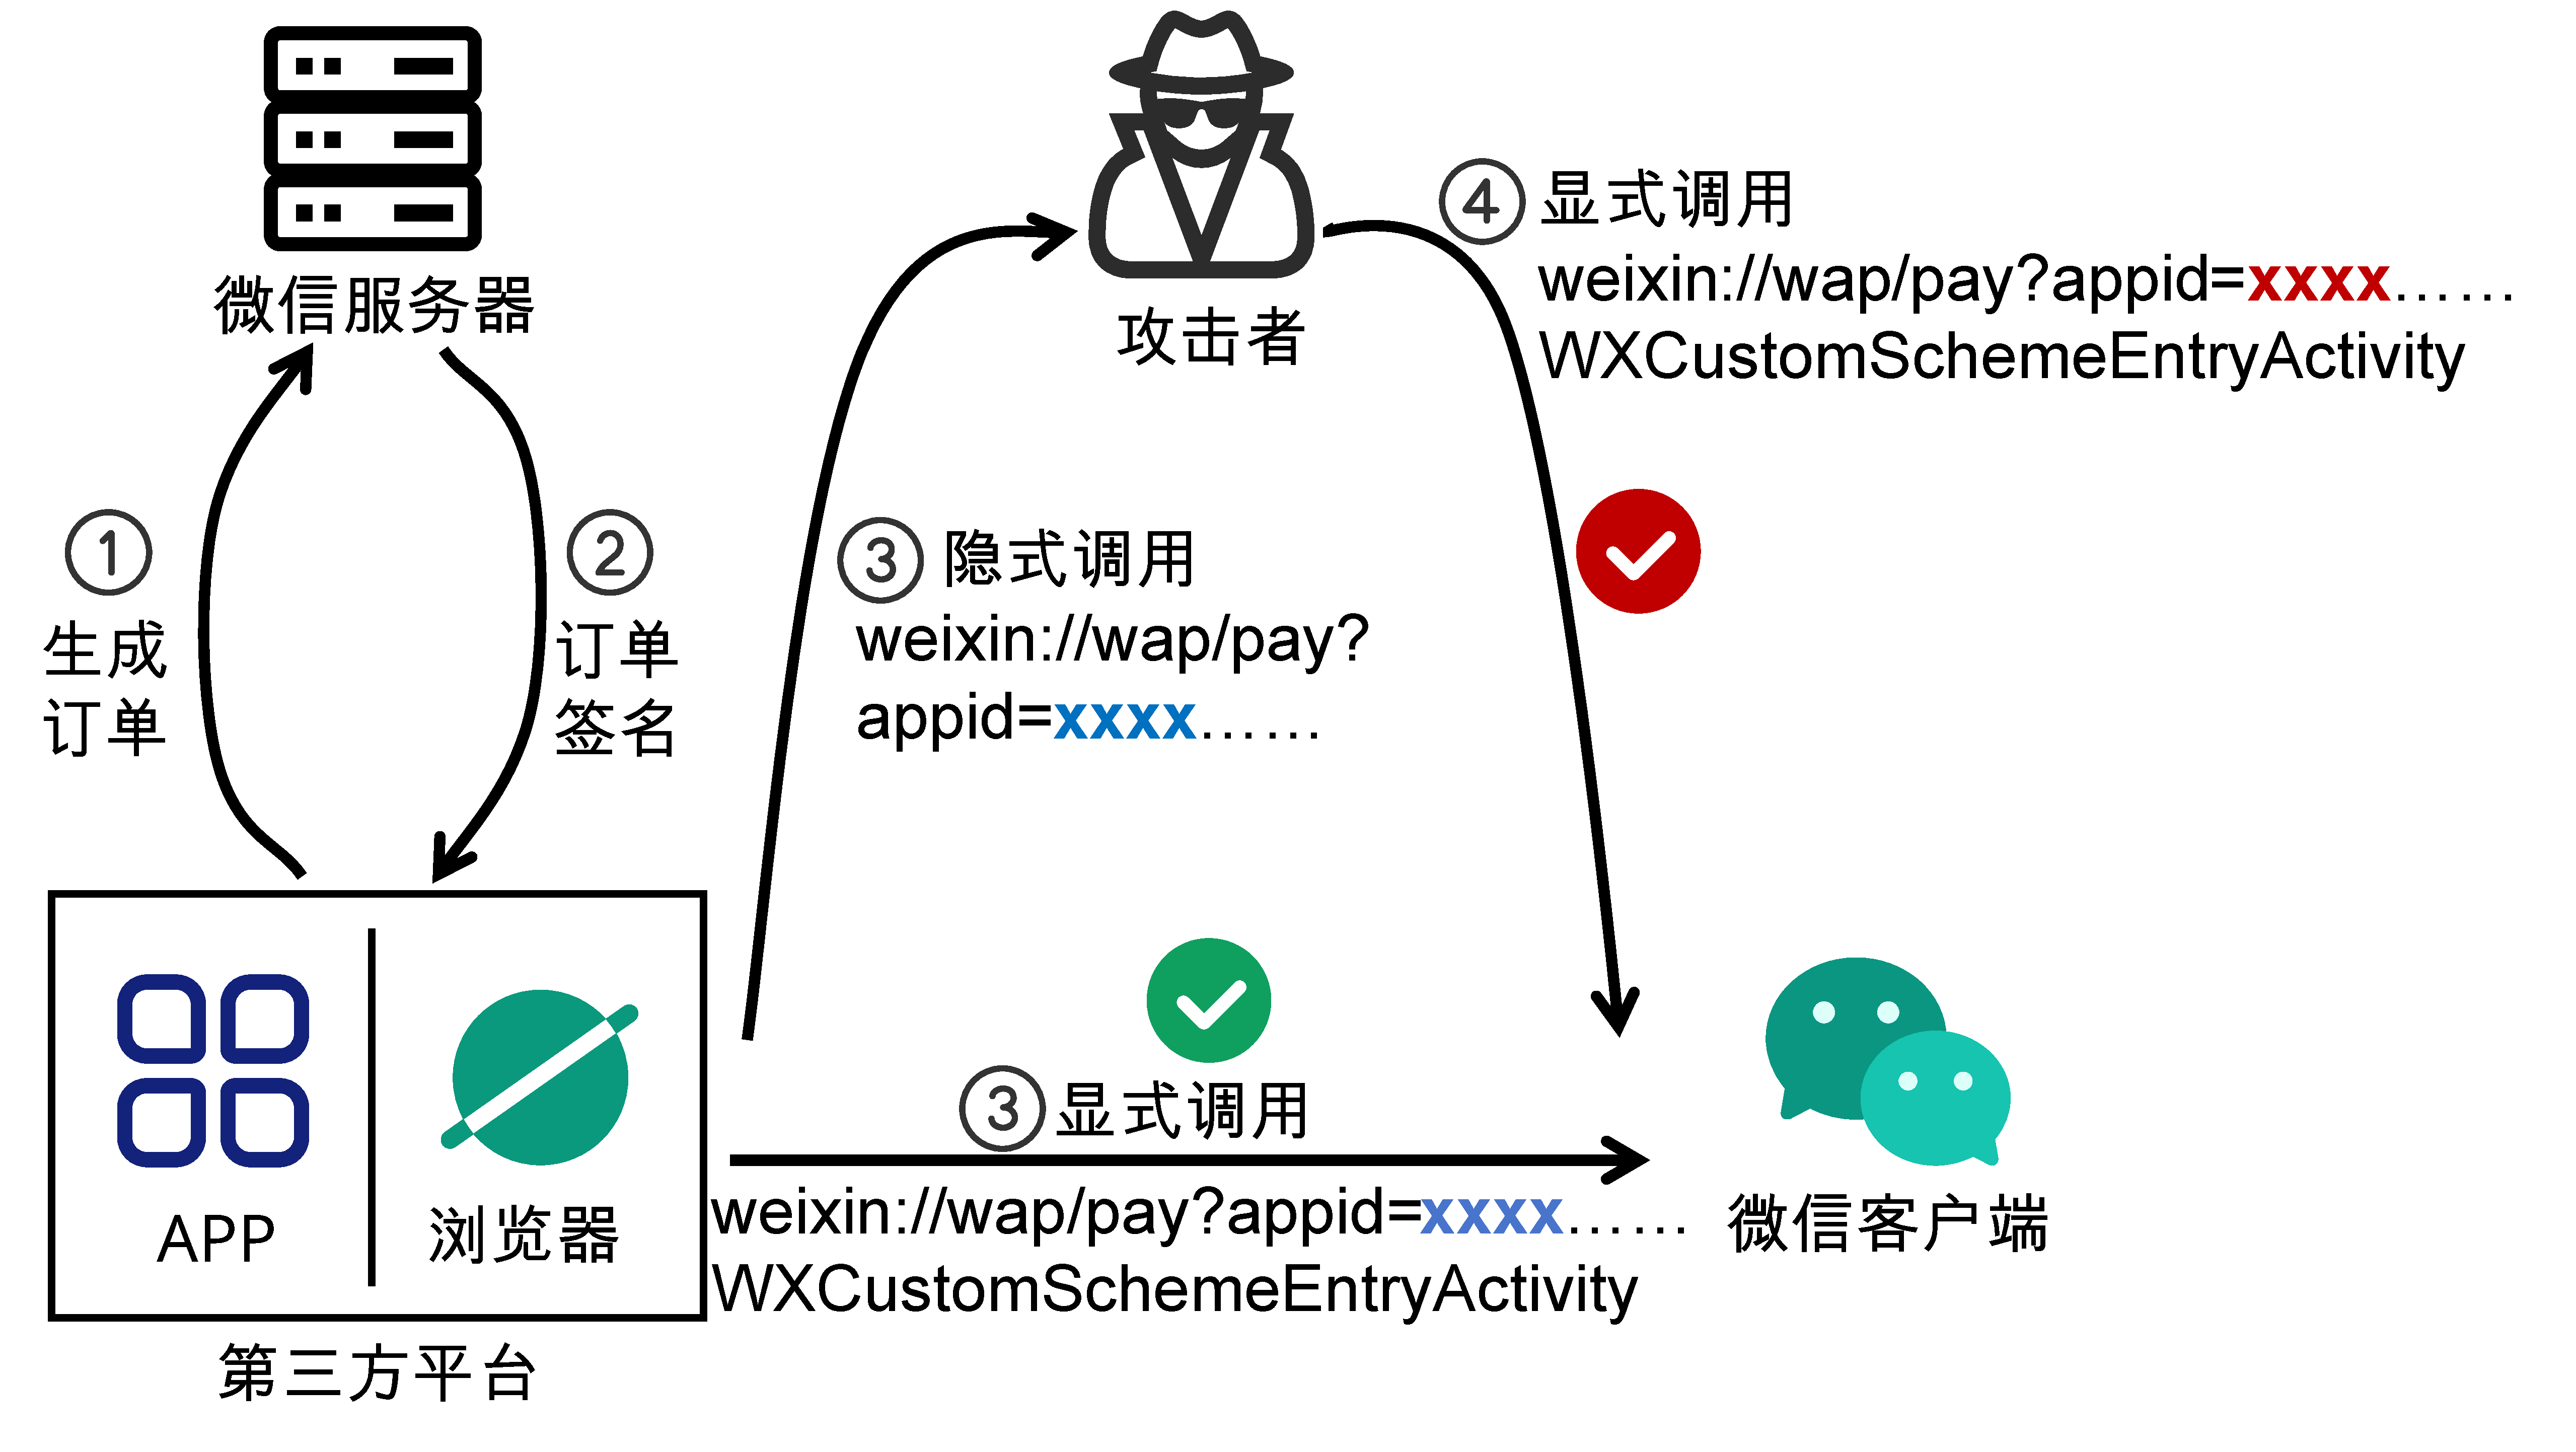
\includegraphics[width=0.97\textwidth]{img/wechat_android_attack.pdf}
    \caption{微信 Android 端支付隐式intent调用劫持攻击示意图}
    \label{fig:wechat_android_attack}
\end{figure}

\subsection{相关工作}
% 分析与论文场景或问题相关的、近三年或经典的研究的不足，并附上相应的参考文献
在第三方支付安全研究领域，Yang等人\cite{YangZLLWZG17-show-me-the-money}首次系统性地研究了Android应用中第三方支付SDK的安全实现问题。
该工作针对国内市场主流的微信支付、支付宝等四种支付SDK，建立了包含七项核心安全规则的多方交互模型。
通过分析7145款应用，研究发现37\%的应用存在支付实现漏洞，主要源于SDK设计缺陷（如密钥硬编码）与商户实现错误（如服务端校验缺失）的耦合问题。
这项工作的重要贡献在于揭示了支付服务商提供的模糊文档和漏洞样本代码会直接导致商户的误用，突破了传统研究中仅归因于商户实现的局限性。

Chen等人\cite{ChenXQL00Z19-devils-in-guidance}则深入研究了支付聚合服务中的逻辑漏洞预测问题。
其提出的Dilution方法创新性地采用自然语言处理技术分析开发者文档，建立了支付流程有限状态机扩展模型。
通过对8家主流聚合服务商的分析，该方法成功预测出41个潜在问题，其中确认了5个高危漏洞。
该研究首次证明仅通过文档分析即可预测设计层面的安全隐患，无需依赖传统的代码审计方法。
研究还量化了安全需求的可执行性，揭示了聚合服务对原始支付安全规则的破坏机制。

形式化方法已在信用卡支付的EMV协议中得到系统应用。
基于Tamarin-prover的符号化建模与验证，研究者揭示并验证了多类协议级漏洞与攻击路径，
包括卡品牌混淆攻击与PIN绕过攻击等\cite{DavidBasin-CardBrandMixupAttack,DavidBasin-PINBypassAttack}，
并对EMV协议开展了更为全面的安全性分析与实践性评估\cite{Radu-Practical-2022,basin_emv_2021}。
这些成果不仅证明了Tamarin在支付协议安全分析中的有效性，也提供了可复用的建模范式与证明技法，为将形式化验证扩展到第三方线上支付场景奠定了方法与工具基础。

\section{意义} 
\subsection{主要挑战}
% 阐述论文方案面临的挑战，建议 200 字以下
\begin{itemize}
    \item \textbf{协议异构与多实体建模挑战}:
        当前第三方支付领域缺乏公开、统一的行业协议标准，各大支付平台均采用各自独立的协议设计。
        同时，同一平台在不同支付场景（如APP内支付、H5支付、小程序支付、扫码支付等）下也使用差异化的协议流程。
        我们需从公开开发者文档提炼可验证的式化模型，但此类文档多面向接入实施，描述偏操作、语义模糊且信息缺漏，增加抽象与语义提取难度。
        此外，用户侧涉及多个交互实体（如商户APP、支付APP、移动浏览器、PC浏览器等），精确捕捉和建模这些多方实体之间的复杂交互关系及其在协议中的角色具有挑战性。
    \item \textbf{现有生态兼容性与修补方案设计挑战}:
        微信支付、支付宝等主流平台已深度融入线上经济活动，支撑着海量交易。
        我们提升安全性的协议修补方案必须具备高度的向后兼容性，方案设计必须严格限制在现有支付流程框架和标准接口规范之内，确保对庞大存量商户和应用的平滑过渡，不能颠覆现有核心业务流程。
        因此，在不扰动现有生态的前提下实现端到端（全链路）安全强化，设计空间受限，具有较大挑战性。
\end{itemize}


\subsection{论文贡献}
% 阐述论文的主要贡献，建议200字以下
\begin{itemize}
    \item 对主流第三方平台支付协议进行形式化建模并使用 Tamarin-prover 验证，证明在不可信终端环境下现有协议无法保证支付安全。
        进一步识别并系统化分析 Android 平台基于 Intent 的支付请求劫持漏洞：恶意应用可篡改支付参数发起欺诈交易。
        进行实验验证，验证该漏洞可被利用，微信和支付宝均受影响。
    \item 计划进行大规模实地调研，评估该漏洞的现实影响力。
        调研 xxx 款手机应用的近 x 个版本支付安全性，发现其中 xxx 款存在支付请求劫持漏洞，根据下载量估算，潜在影响用户数达 xxx 万，表明该漏洞具有广泛性。
    \item 提出兼容现有生态的协议修补方案：在注册阶段建立共享密钥，支付阶段利用该密钥保护订单完整性并实现双向认证，从根本上阻断支付请求篡改。
        对该方案进行形式化建模，并用 Tamarin-prover 证明其满足既定安全属性，具备支付全链路安全保障能力。
\end{itemize}


\section{方案}
\subsection{安全模型}
% 描述敌手能力和目的
本安全模型针对第三方支付平台的在线支付场景，涉及用户（User）、商家（Merchant）和支付系统（Payment System）三个主要的实体。
用户通过不同的终端（如商户APP、移动浏览器、PC浏览器等）发起向商户提交订单。
商户根据订单，向支付系统提交支付请求，并向用户返回支付信息（如二维码、支付链接等）。
支付系统负责处理支付交易并与商户和用户进行交互。
 
在本模型中，攻击者的\textbf{威胁模型}如下： 
\begin{compactitem}
    \item \textbf{恶意应用控制：} 攻击者已在用户智能手机上植入并运行恶意应用，能够发起主动攻击，篡改由任何商家终端发起的、调起支付软件的所有支付信息。
    \item \textbf{通信中间人攻击：} 假设用户未接入安全网络，攻击者可监听并篡改用户设备与商户服务器之间的全部通信数据。
\end{compactitem}

同时，我们做出以下\textbf{安全假设：}
\begin{compactitem}
    \item \textbf{支付系统整体安全：}
        我们假设支付系统本身是安全的，即支付服务器与支付APP之间的通信信道完全可信，具备机密性与完整性保护，攻击者无法篡改二者之间的直接通信数据。
        因此，可将支付服务器与支付APP视为一个统一的整体，统称为``支付系统''。
    \item \textbf{支付接口安全：}
        我们假设支付系统为商户提供的 API 已被正确配置与使用，商户服务器与支付系统之间的通信同样安全，攻击者无法篡改该通道中的数据，通信的机密性与完整性得到保障。
\end{compactitem}


\subsection{解决方案}
% 陈述论文的具体方案
添加注册阶段，商家与用户在注册阶段共享 $CMK$，流程如图\ref{fig:register}所示。
\begin{figure}[h]
    \centering
    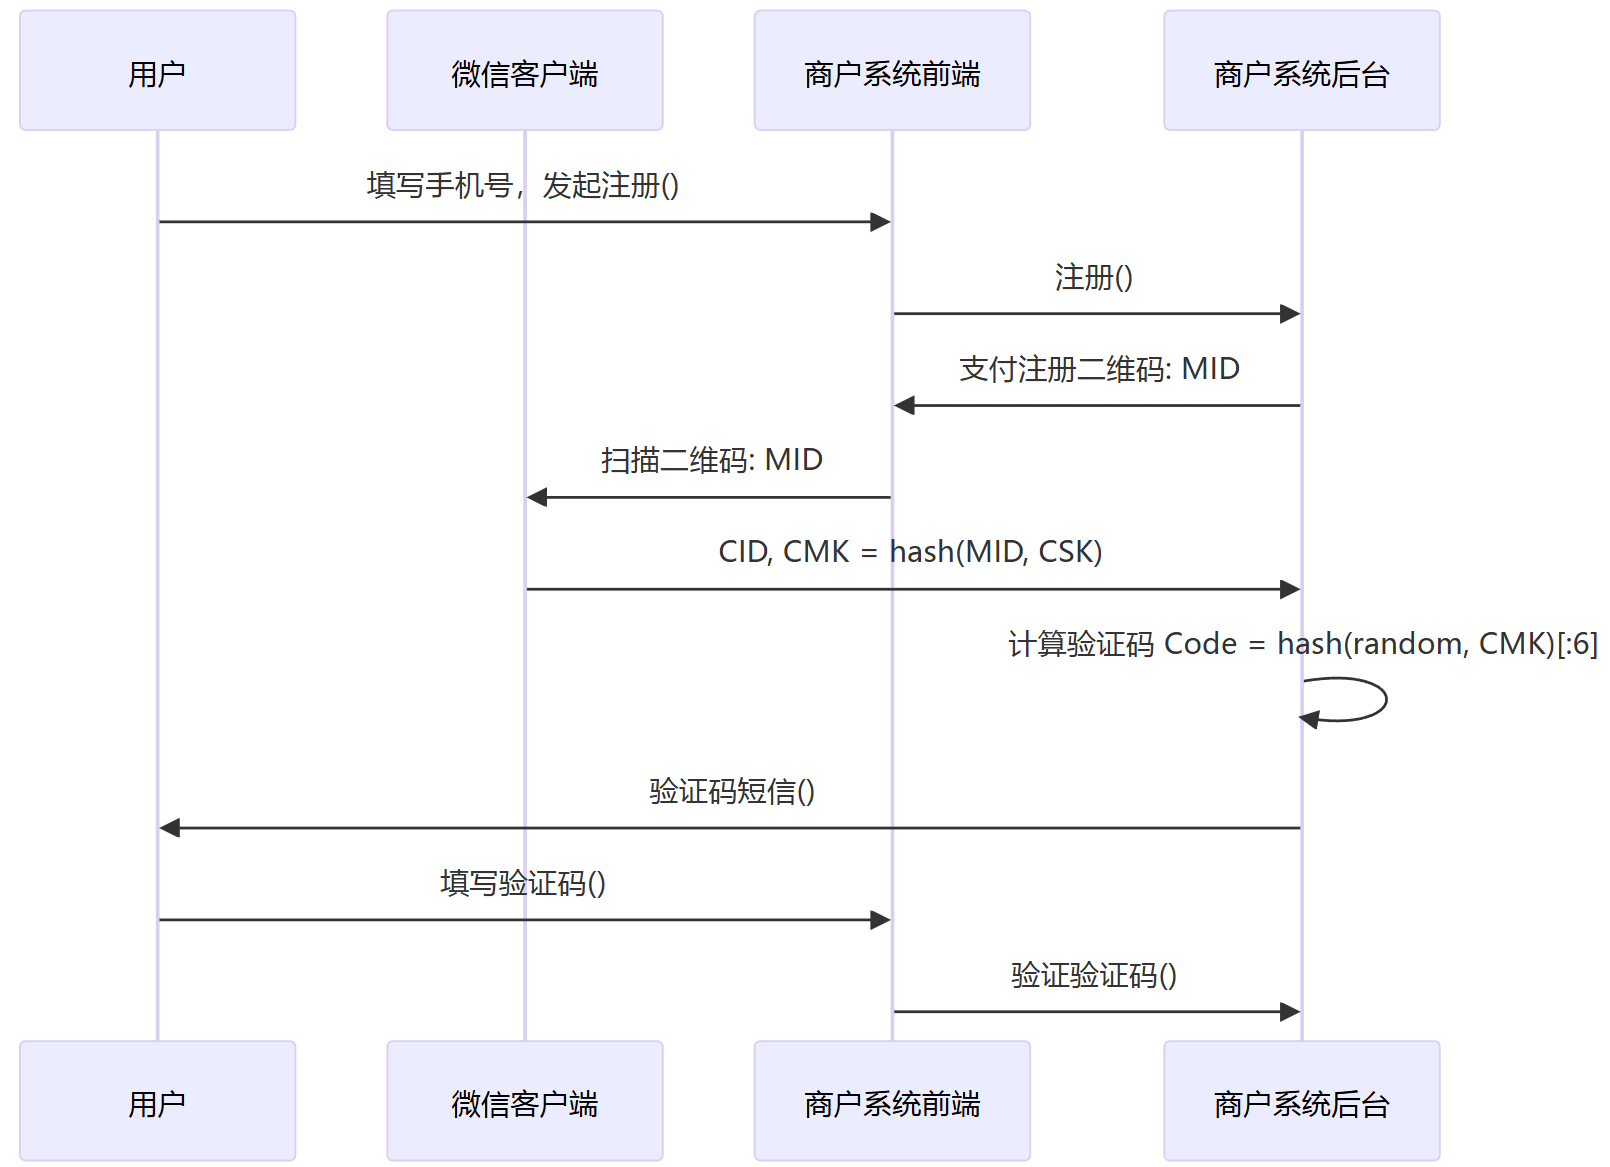
\includegraphics[width=0.8\textwidth]{img/reg.png} 
    \caption{注册阶段}
    \label{fig:register}
\end{figure}


在支付阶段利用  $CMK$ 保护订单完整性和双向认证，流程如图\ref{fig:pay}所示。
\begin{figure}[!h]
    \centering
    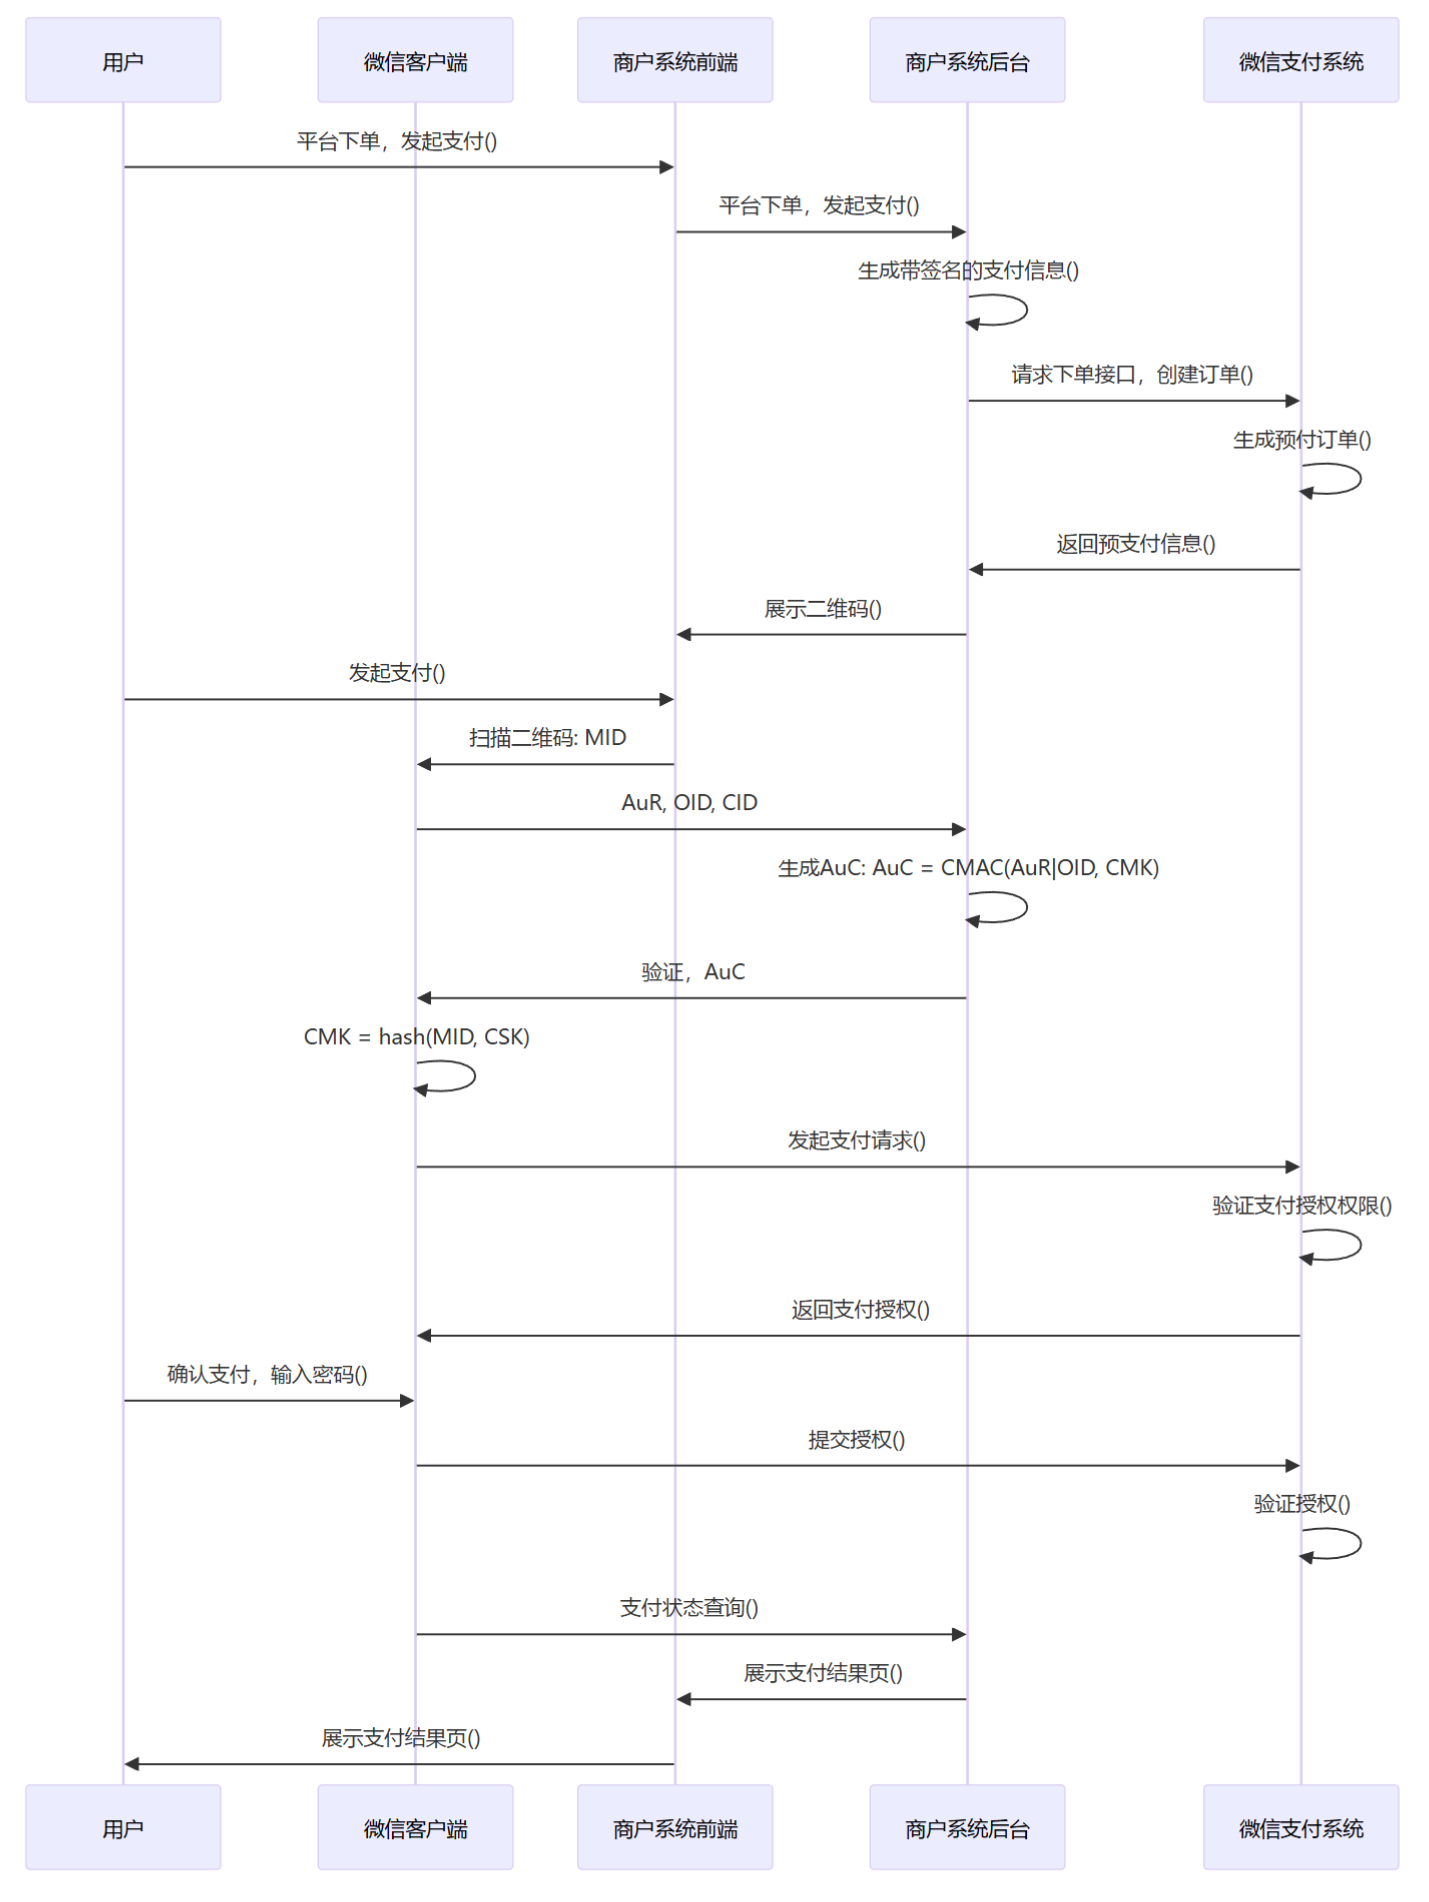
\includegraphics[width=0.8\textwidth]{img/pay.png}
    \caption{支付阶段}
    \label{fig:pay}
\end{figure}


\section{评估}
\subsection{评价标准}
% 列出评价论文方案的理论或实验标准
使用Tamarin-prover对现有协议和修补方案进行形式化验证，验证其是否满足定义的安全属性。


\bibliographystyle{unsrt}
% \bibliographystyle{plain}
\bibliography{library}

\end{document}